%----------------------------------------------------------------------------%
\chapter{Carbon Nanotubes}
%----------------------------------------------------------------------------%
\begin{figure}[htb!]
	\centering
	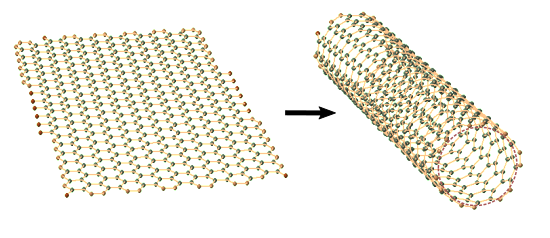
\includegraphics[width=0.8\textwidth]{./Figures/CNTs/graphine_cnt.png}
	\caption{A sheet of graphene is rolled to form a (7, 5) chirality CNT. Graphene and CNT  images were rendered using Dr. Shigeo  Maruyama's  "Nanotube Coordinate Generator" program \cite{maruyama2}.}
	\label{fig:grahine_cnt}
\end{figure}
First discovered by S.Iijima and T. Ichihashi in 1993, carbon nanotubes (CNTs) are single layers of graphene rolled up into a hollow cylinder near 1nm in diameter and average near 1$\mu$m in length. Due to the extreme diameter to length ratio, their geometry allows them to be treated as a 1D material. CNTs possess unique optical properties that have found a wide range of applications\cite{yamashita}. Their most important application to us is the lack of photobleaching and the fact that they do not degrade in water, solving the main permanence issues with using fluorescent dyes like ICG. In this section follows a description of the attributes that make them attractive from an optical standpoint, going over their characterizing properties, nonlinear optical properties, and fluorescence.
\section{Characterizing Carbon Nanotubes}
\begin{figure}[htb!]
	\centering
	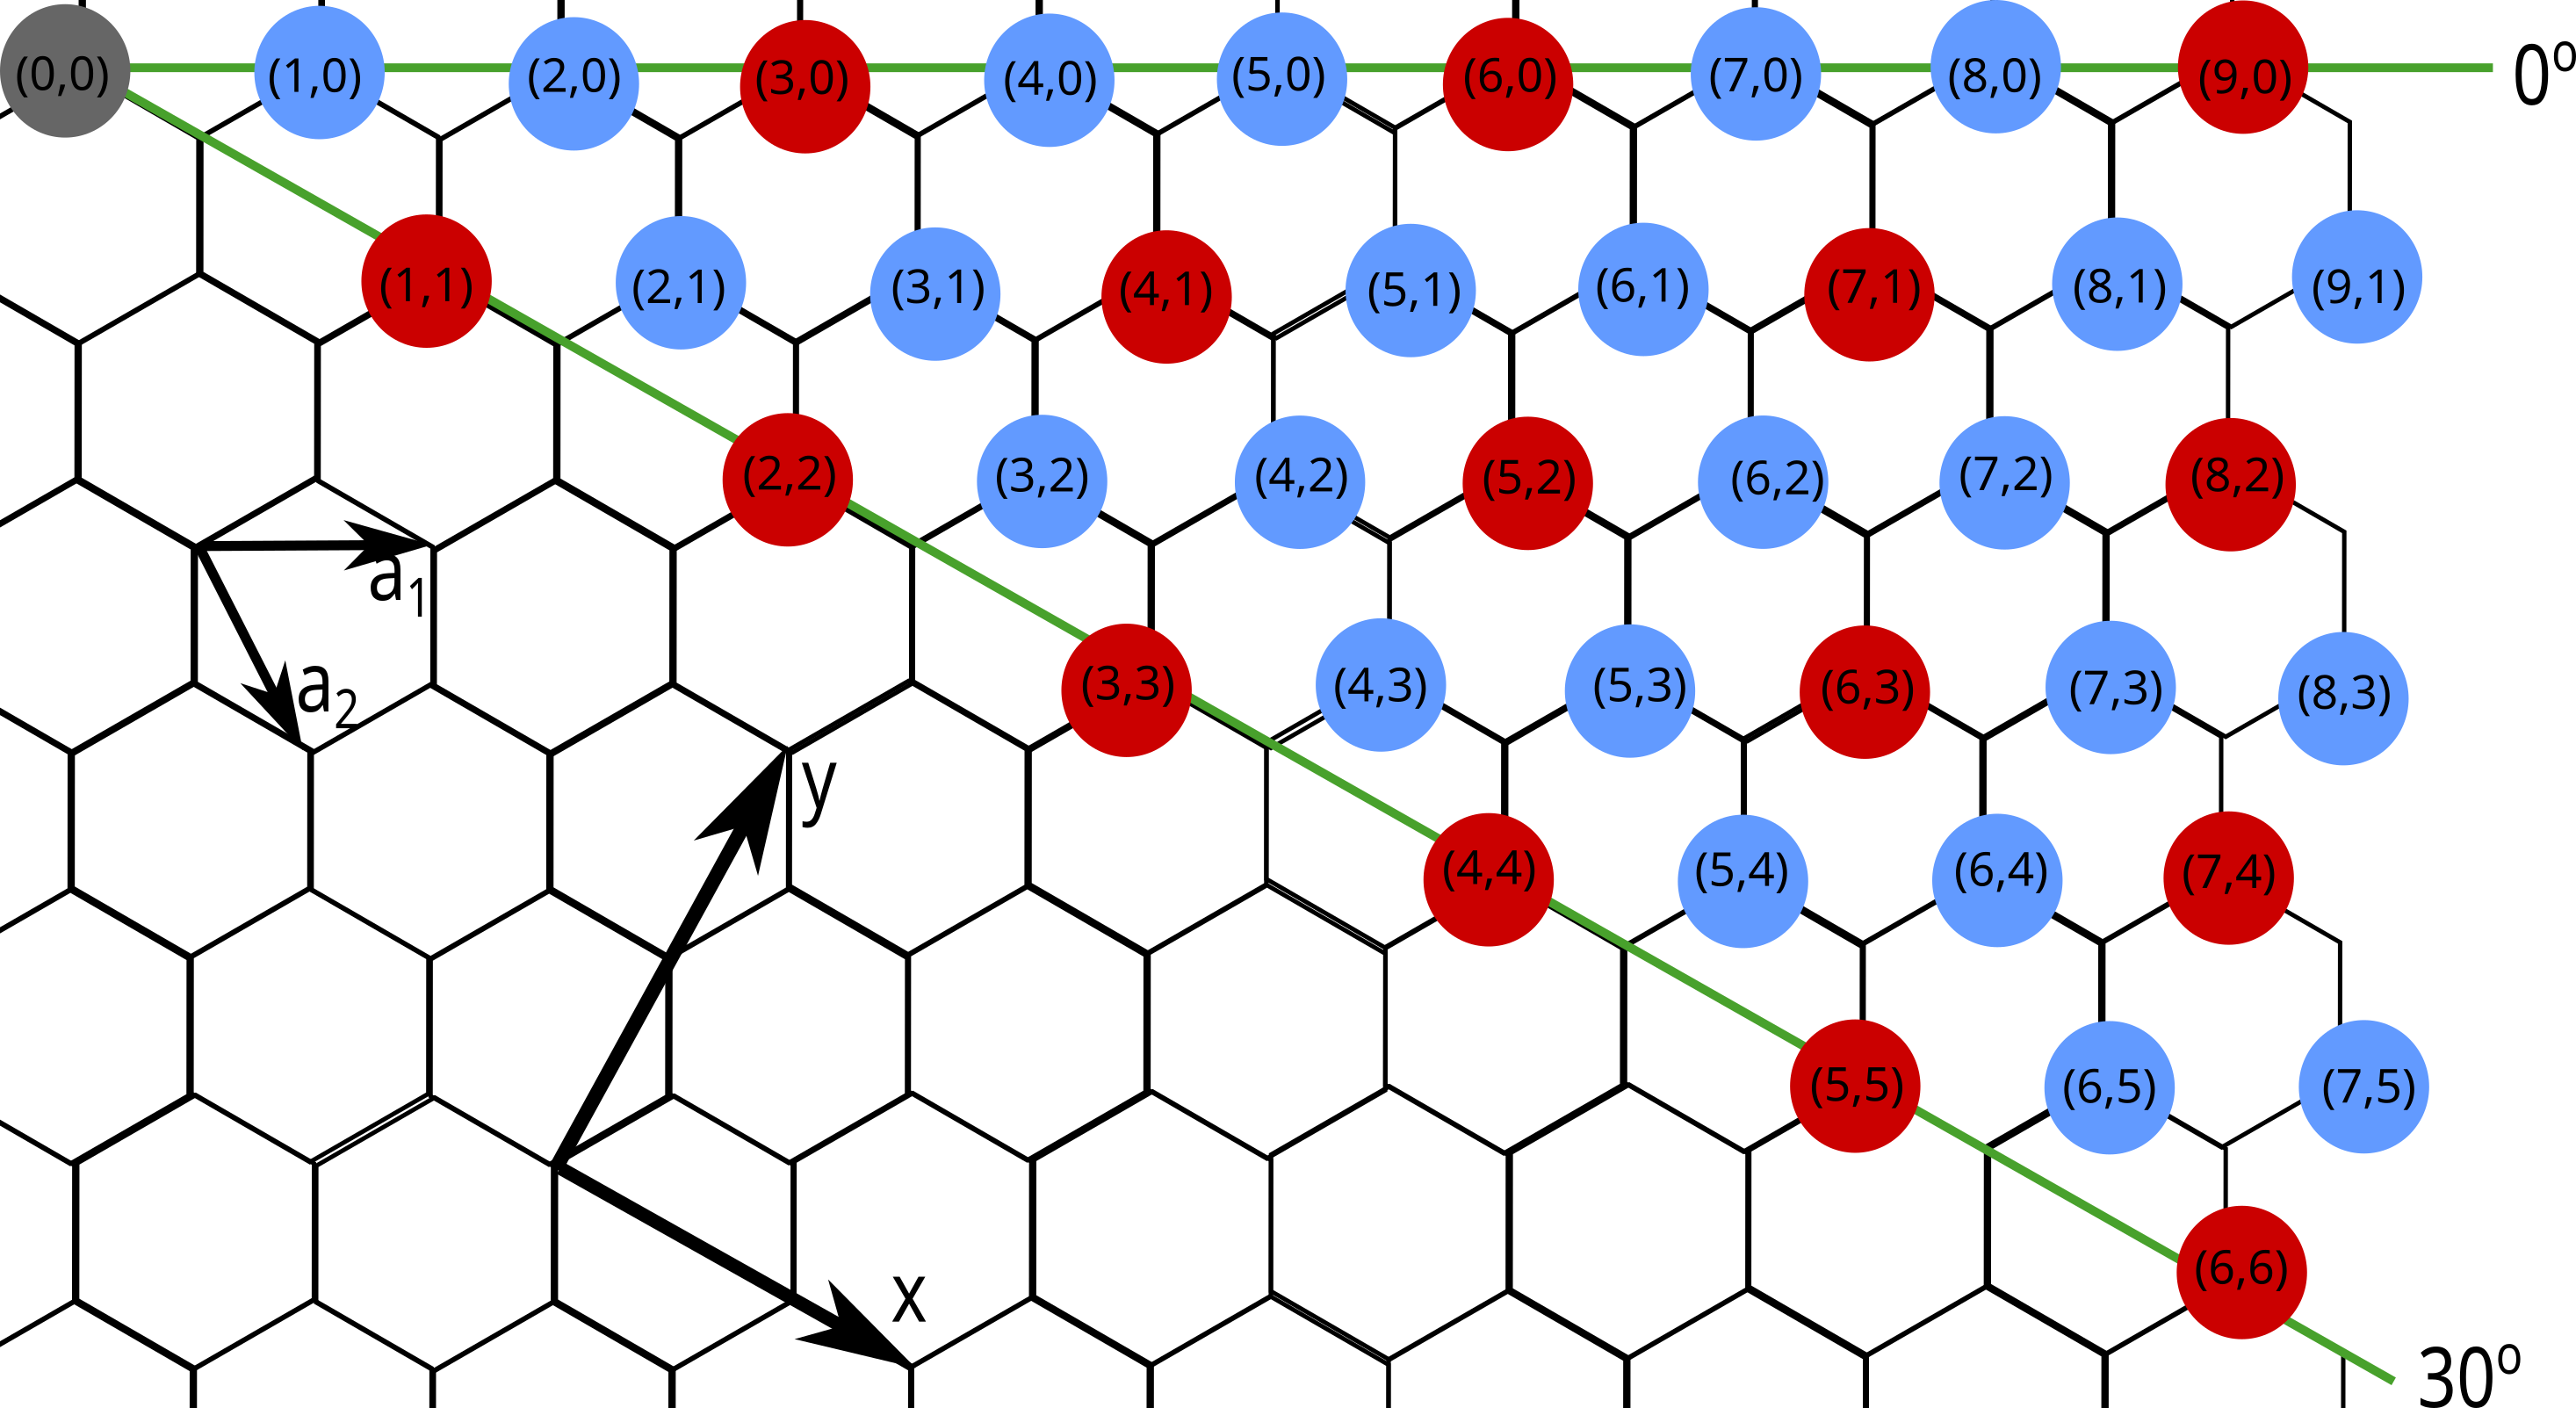
\includegraphics[width=0.8\textwidth]{./Figures/CNTs/chiral.png}
	\caption{Chiralities of CNTs with red dots indicating metallic and blue dots semiconductors. }
	\label{fig:chiralities}
\end{figure}
The main descriptive property of CNTs is the chiral vector, the inter-valued scaling of the unit vectors for the honeycomb structure of graphene, written in the form (n, m).
\begin{equation}
	C_h = na_1 + ma_2 = (n, m)
\end{equation}
The unit vectors describing the lattice are of equal length and in Cartesian coordinates are defined
\begin{equation}
	a_1 = (\frac{\sqrt3}{2}, \frac{1}{2})\sqrt{3}a_{C-C}\\
	a_2 = (\frac{\sqrt3}{2}, -\frac{1}{2})\sqrt{3}a_{C-C}
	\label{unit_vecs}
\end{equation}
 where $a_{C-C}$ is the length of the carbon bond. For graphene, $a_{C-C}$=1.421 (\AA) but for CNTs is approximately 1.44(\AA) with variation coming from the tube curvature\cite{saito}. From the chiral vector, much about the electronic and optical properties of individual CNTs can be inferred. The angle between the unit vectors, known as the chiral angle $\theta$, gives the direction of the chiral vector and the diameter,$d_t$, of the CNT are related to the chiral numbers:
\begin{equation}
	\theta = tan^{-1}\Bigg[\frac{m\sqrt{3}}{m + 2n}\Bigg]
\end{equation}
\begin{equation}
	d_t = \frac{a_{CC}\sqrt{3}}{\pi} \sqrt{n^2 + nm + m^2}
\end{equation}
The chiral angle is typically defined between 0${}^\circ$(a "zigzag" configuration) and 30${}^\circ$(an "armchair" configuration), labeled in Fig.\ref{fig:chiralities} due to the six-fold rotational symmetry lattice, as CNTs of mirrored chiral angles will have the sample opto-electrical properties. \\
As can be seen from the above definition, the tube diameter of CNTs is quantized. This quantization stems from the additional electron confinement around their circumference
\begin{equation}
	C_h\cdot\kappa = 2\pi q
\end{equation}
 as the cutting joining of the edges of graphene form the tubes only occurs at lines intersecting the lattice vertices. $\kappa$, the cutting line along the graphene energy bands, at integer value $q$ positions forms a the corresponding pattern of  metallic or a semiconductors \cite{dresselhaus} with all CNTs with a difference in chiral numbers $|m-n|$ that are multiples of 3 emerging as metallic. Work by H. Kataura et. al \cite{kataura} first plotted the energy differences between the van Hoven transitions, corresponding to the peaks in the conduction and valence bands enumerated starting from the Fermi energy, indicated in the 1D DOS plots in Fig.\ref{fig:kataura}(b)(c) later determined from \cite{saito}. The relationship of the first van Hoven transition to the diameter is found to be 
 \begin{equation}
 	E_{11} = \frac{2\gamma a_{C-C}}{d}
 \end{equation}
 is shown in Fig.\ref{fig:kataura}(a), with the average band gap energies split along semiconductor and metallic chiral values. The absorption peak wavelength of a nanotube sample is determined by the mean tube diameter, and the absorption spectral bandwidth will be determined by the tube diameter distribution of the CNT sample.
\begin{figure}[h]
	\centering
	\foreach \x \y in {kautura/0.7, dos\_66/0.47, dos\_76/0.47}
	{
		\begin{subfigure}[b]{0\y\textwidth}
			\includegraphics[width=\textwidth]{./Figures/CNTs/\x.png}
			\caption{}
		\end{subfigure}
		\hfil
	}
	\caption{(a)The Kataura plot, showing the relationship between CNT diameter and energy separation. Red dots indicate metallic and black semiconducting. The density of states for (b) Metallic and (c) Semiconducting CNTs and their energy band gaps. The green line indicates the Fermi level. Plots generated using data from\cite{maruyama}.}
	\label{fig:kataura}
\end{figure}
\clearpage
\subsubsection{Polarization Dependence}
Single isolated CNTs exhibit polarization dependence with the electric field in optical selection rules, i.e. the possible transitions from one quantum state to another \cite{thomsen}. Polarization dependence is only strong in zigzag-type nanotubes, the parity of the  dipole operator ( -1 in the horizontal plane dipole operator along the z-axis and +1the x-y plane) thus indicates absorption of light with the optical polarization parallel to the axial direction of the tube. However, in a bundle or random-oriented CNT grouping there will be no polarization dependence and it is not something that is of concern in CNTs dispersed in a solution.

\section{Nonlinear Optical Properties of CNTs}
The general relationship between the polarization and electric field of a material is defined \cite{yamashita} as
\begin{equation}
	P(t) = \epsilon_0(\chi^{(1)}E(t) + \chi^{(2)}E^2(t) + \chi^{(3)}E^3(t)+...)
\end{equation}
where $\chi^{(1)}$ is the linear susceptibility and $\chi^{(2)}$ and $\chi^{(3)}$are the second and third order susceptibility. Due to symmetry of the CNT’s structure, the second-order susceptibility is zero but a large third-order nonlinearity in CNTs has been measured \cite{martinez} and is theorized to be a product of the one dimensional motion of the delocalized $\pi$-band electrons at a fixed lattice ion configuration \cite{margulis}.  The third-order nonlinearity is responsible for the saturable absorption $\alpha$ of a material as well as the nonlinear Kerr effect.
The refractive index for such a material will be composed of the real part of the third-order susceptibility with $I$ defining the optical intensity, $n_0$  as the linear refractive index, $n_2$ and  is the nonlinear refractive index.
\begin{equation}
	n = n_0 + n_2I = n_0 + \frac{3Re[\chi^{(3)}]}{4\epsilon_0cn_0^2}I
	\label{eq:refractive_index}
\end{equation}
Saturable absorption is a phenomenon where high intensity light will reduce the absorption of a material, but at weak intensity, the light will be absorbed and cause attenuation. This property of materials with strong third-order susceptibility like CNTs can be used to filter out weaker optical signals in noisy optical pulses, while simultaneously allowing strong pulses to pass through. The absorption coefficient is composed of the imaginary part of the third-order susceptibility and $\alpha_0$, $\alpha_{int}$, and $\omega$ are the linear absorption coefficient, the non saturable absorption coefficient, and optical angular frequency respectively:
\begin{equation}
	\begin{aligned}
	\alpha &= \frac{\alpha_0}{1+\frac{I}{I_S}} + \alpha_{int}\\
	&\sim\alpha_0 + \alpha_{int} + \frac{3\omega Im[\chi^{3}]}{2\epsilon_0c^2n_0^2}I
	\end{aligned}
	\label{eq:absorption_coefficient}
\end{equation}
the saturation intensity $I_s$ is the power per unit area it takes in a steady state to reduce the absorption to half of completely saturated value, referred to as the unbleached state. Saturable absorption is observed in all materials with optical absorption resulting from electron transition between two energy levels \cite{thomsen}, but it is rare to find materials that have a recovery time that has a fast recovery time compared to the pulse duration. In bundles of  CNTs  with a variety of diameter sizes, entanglement between semiconducting and metallic via electrons tunneling and coupling from semiconducting CNTs to metallic CNTs \cite{gambetta} can result in picosecond to femtosecond range recovery time. Bundled CNTs have found application in  in ultra-fast laser applications where this sort of recovery time is needed, having been successful implemented in mode-locking femtosecond fiber-lasers\cite{fl1, fl2, fl3, fl4}. 

\section{Fluorescence of CNTs}
Arriving at the interest in CNTs for this thesis, semiconducting CNTs can be optically excited and emit fluorescence\cite{hendler} when well-dispersed. Bundled CNTs or placed on a substrate have little to no fluorescence at all, as interactions between CNTs cause increased quenching effects, the highest fluorescence quantum yields are seen in CNTs suspended in aqueous solutions. Though certain solvents mix better with certain chiralities CNTs to increase fluorescence, isolation to single chiralities one of the largest factors in increasing fluorescence. Desired type of CNTs can be targeted and isolated in a single step using modified aqueous two-phase extraction(ATPS)\cite{turek}.In this process, hydration modulating agents are mixed in to solutions to tune the arrangement of surfactants on their surface. Depending on the mixture, selected CNTs turn highly hydrophobic or hydrophilic, separating them from the rest of the mixture.\\
Fluorescence in carbon nanotubes is the product of absorption at the excitation frequency, corresponding to the second Van Hove optical transition (E22), labeled in Fig.\ref{fig:kataura}(c), from the valence to conduction bands, followed by relaxation to the first Van Hove optical transition (E11) from the conduction to valence band. The corresponding excitation and emission  wavelengths can be as a function of diameter in nanometers and chiral angle are degrees derived in \cite{bachilo}. The parameters fitted differ along CNT groups, having to do with chiral number differences:  (n-m) mod 3 = 1 is group 1, (n-m) mod 3 = 2 is group 2,  (n-m) mod 3 = 0 are metallic CNTs and do not fluoresce and so are excluded. \\
For group 1:
\begin{equation}
	(Emission)\lambda_{11} = \Bigg[\frac{10^7(cm^{-1})}{157.5+1066.9d_t} - A_{1m1}(cm^{-1})\frac{cos(3\theta)^{1.374}}{d_t^{2.272}} \Bigg]^{-1}
\end{equation}
\begin{equation}
	(Excitation)\lambda_{22} = \Bigg[\frac{10^7(cm^{-1})}{145.6+575.7d_t} + A_{2m1}(cm^{-1})\frac{cos(3\theta)^{0.828}}{d_t^{1.809}} \Bigg]^{-1}
\end{equation}
For group 2:
\begin{equation}
	(Emission)\lambda_{11} = \Bigg[\frac{10^7(cm^{-1})}{157.5+1066.9d_t} + A_{1m2}(cm^{-1})\frac{cos(3\theta)^{0.886}}{d_t^{2.129}} \Bigg]^{-1}
\end{equation}
\begin{equation}
	(Excitation)\lambda_{22} = \Bigg[\frac{10^7(cm^{-1})}{145.6+575.7d_t} - A_{2m2}(cm^{-1})\frac{cos(3\theta)^{1.110}}{d_t^{2.497}} \Bigg]^{-1}
\end{equation}
Additional parameters $A_{1m1}, A_{1m2}, A_{2m1}, A_{2m2}$, account for variations of spectrum in same diameter CNTs. Not all variation differences are yet explained but comparison of aqueous solutions\cite{turek}\cite{weisman} found spectral shifts of $\sim$2\%. \\
Plots of the excitation-emission spectrum are using variational parameters from fitting to data of samples of individual SWNT in aqueous sodium dodecyl sulfate (SDS)\cite{weisman} are shown in Fig.\ref{fig:cnt fluorescence}. Group 1 CNTs have lower Stokes shifts, and small chiral angles ($< 2^\circ$) while group 2 have higher Stokes shift and span full $0^\circ$to $30^\circ$ chiral angle range with similar angles along chiral number difference $(n - m)$. Regardless of group, the in excitation and emission wavelengths increase with diameter.

\begin{figure}[h]
	\centering
	\foreach \x in {degrees, diameter}
		{
			\begin{subfigure}[b]{0.49\textwidth}
				\includegraphics[width=9cm, height=8cm]{./Figures/CNTs/\x.png}
				\caption{}
			\end{subfigure}
			\hfil
		}
	\caption {Group characteristics of CNTs colored by using variational parameters from\cite{weisman}, valid for diameters $>0.5nm$. Color spectrum of plot denoting (a)chiral angle and (b)diameter. Increase in Stokes shifts with diameter along chiral difference $(n - m)$ lines, noted in red and connected by black lines.}
	\label{fig:cnt fluorescence}
\end{figure}
\clearpage